\chapter{Flutter Implementation}
\label{chapter:05}
The final product allows the programmer to compute mobility features with the following 3 lines of code displayed in Figure \ref{fig:code-example-intro}. This chapter will describe how the package design described in Chapter \ref{chapter:04} was implemented in Flutter such that this succinct code interface was achieved.  The Flutter, and Python source code for this thesis can be found at \url{https://github.com/thomasnilsson/mobility-features-thesis}.

\begin{figure}[h]
    \centering
    \begin{minted}{dart}
    /// Collect data with a location plugin
    List<LocationSample> locationSamples = ///

    /// Store data via the package
    await ContextGenerator.saveSamples(locationSamples);
    
    /// Compute Features via the package
    MobilityContext context = await ContextGenerator.generate();
    \end{minted}
    \caption{All the three lines of code necessary for the application developer to write}
    \label{fig:code-example-intro}
\end{figure}



\section{Flutter, Packages and Plugins}
Flutter is a cross-platform app development framework developed by Google and released in 2018. It allows an application programmer to write a mobile application using a single codebase written in the Dart programming language, and compile this source code to a native Android and iOS application. This has the clear advantage of reducing the amount of labour needed to produce mobile applications which most of the time need to be released on both platforms. Packages and Plugins are the Flutter equivalent of a software library which is hosted on the Dart package manager at \url{pub.dev}, the Mobility Features Package is hosted at \url{pub.dev/packages/mobility_features}. 

\subsection{Why Flutter?}
It was chosen to implement the package in Flutter for several reasons: Firstly it is cross-platform, meaning the same code base can compile to both Android and iOS. For this reason one could also have chosen other frameworks such as React Native\footnote{\url{https://reactnative.dev/}} developed by Facebook. The author was employed at CACHET who uses Flutter for mobile development. An example of a CACHET PhD project is \cite{mubs-rohani}. In addition, the author had already authored many packages\footnote{\url{https://pub.dev/publishers/cachet.dk/packages}} for the CARP Mobile Sensing Framework by CACHET.

\subsection{Packages and Plugins}
A flutter \textit{package} is a library containing Dart pure code that enables the creation of modular code that can be shared easily. A package declares the package name, version, author, and so on (see Figure \ref{fig:pubspec}, and secondly a source code directory named \verb|lib|. It is relevant to develop a package when common functionality is to be shared among applications, and the functionality can be computed in the Dart programming language alone. The \textit{Mobility Features Package} is a Flutter package that contains a collection of algorithms that provides an application programmer with object-oriented abstractions that allows him/her to calculate relevant features for a mobile health application. 

Whenever a functionality is wanted which is only available through a native API, such as the camera or battery level, a \textit{plugin} is used instead. In contrast to a package, a plugin contains three codebases: Flutter (Dart), Android (Kotlin/Java), and iOS (Swift/Objective C). The Dart codebase contains an implementation which can be called from a Flutter app, and in turn calls the implementation in the Android environment and the iOS environment (whichever platform the device runs). It does so by transporting data between the platforms, which means no real computation is performed in the Dart environment; the Dart implementation simply invokes a method in the native environment, the native environment performs the computation, or data collection, and then sends back an answer. For transporting data between the native environment and the Dart environment, messaging channels are used, namely \textit{MethodChannels} and \textit{EventChannels}. A \textit{MethodChannel} is used for communicating when data is to be transferred on a whenever a method is invoked. In contrast to this, the \textit{EventChannel} allows streaming data from the native environment every time an event is triggered in the native environment, such as when a sensor picks up on a new data point. A Location API plugin which streams location data continuously uses an \textit{EventChannel}.

This method invocation library is referred to as a \textit{plugin} within the Flutter world, in contrast to a \textit{package} which simply invokes other Dart code and as such contains no platform-specific source code.  The Location API, available on both iOS and Android, will not be invoked directly from this package since that would require it to be a plugin. This has two main upsides: From the point of the application developer, it allows him/her to use their location plugin of choice (of which there are many \footnote{\url{https://pub.dev/packages?q=location}} with specific parameters for how the location is tracked (ex frequency and distance). Secondly, from the perspective of the maintainer of this package, the package becomes much more modular and in turn easier to maintain.

\subsection{Package Structure}
The package contains two main directories and three metadata files as depicted in Figure \ref{fig:package-structure}. The first directory is the source code directory, \textit{lib}, containing the domain model, and algorithms for computing MobilityContexts. The second directory is the \textit{test} directory containing unit tests which aid in the process of validating the algorithms. The metadata files are the \textit{CHANGELOG.md} which contains a list of changes made to the package such that an application programmer can keep track of changes to the API. 

\begin{figure}
    \centering
    \begin{verbatim}
        mobility_features
        ├── lib/
        │   ├── mobility_context.dart
        │   ├── mobility_domain.dart
        │   ├── mobility_features.dart
        │   ├── mobility_functions.dart
        │   ├── mobility_intermediate.dart
        │   └── mobility_serializer.dart
        ├── test/
        │   ├── data/
        │   ├── mobility_features_test.dart
        │   └── test_utils.dart
        ├── CHANGELOG.md
        ├── pubspec.yaml
        ├── README.md
    \end{verbatim}
    \caption{The file structure of the Mobility Features Flutter Package}
    \label{fig:package-structure}
\end{figure}

The \textit{pubspec.yaml} contains the package specification including the package name, a description, version, homepage, and a list of dependencies. The dependencies are a the package on which the package depends, as in this case the Mobility Features Package depends on the \verb|simple_cluster|, \verb|stats| and \verb|path_provider| packages each with a specific version number. The package itself also has such a version number which allows an application developer to import a specific version of the package, for example if they built their application around a previous release, they may wish to continue depending on that specific release rather than upgrading to the newest version.

\begin{figure}
    \centering
    \begin{minted}{yaml}
        name: mobility_features
        description: Real-time mobility feature calculation
        version: 1.1.5
        homepage: https://github.com/cph-cachet/flutter-plugins/
        
        environment:
          sdk: ">=2.7.0 <3.0.0"
        
        dependencies:
          flutter:
            sdk: flutter
          simple_cluster: ^0.2.0
          stats: ^0.2.0+3
          path_provider: ^1.6.10
        
        dev_dependencies:
          flutter_test:
            sdk: flutter
    \end{minted}
    \caption{The pubspec.yaml file for the Mobility Features Package}
    \label{fig:pubspec}
\end{figure}

Lastly, the README.md file contains instructions for using the package including code snippets and use case examples. 

\subsection{Dart Libraries}
The Mobility Features Package has a library file of the same name as the package \textit{mobility\_features.dart} which is the central point of import statements for all the source code. All import statements are made within this file, and each file belonging to the library are declared using the \textit{part} keyword and. 

\begin{minted}{dart}
    library mobility_features;
    
    import 'dart:math';
    ...
    
    part 'mobility_functions.dart';
    ...
\end{minted}

Each file included in the library will have the equivalent \textit{part of} keyword at the top of their file, which allows the file to import all dependencies from the library, and makes the file public to other files within the library and vice versa.

\begin{minted}{dart}
    part of mobility_features;
    ...
\end{minted}

Classes and field which are private and still visible internally to other classes within the library. This helps making things communicate internally but have closed private access to the application programmer, for reasons discussed in Chapter \ref{chapter:04}

\subsection{Package Publishing}
Distributing a Flutter package is done via the Dart Package Manager, Pub. Pub is essentially a a git repository of a package including all versions of that package. When publishing a package the contents of the README file are converted to HTML and is what the user is initially presented with. The README should therefore give a brief overview and description of the package, in addition to instructions. Figure \ref{fig:pub-package} shows the latest version of the package hosted at \url{https://pub.dev/packages/mobility_features}.

\begin{figure}
    \centering
    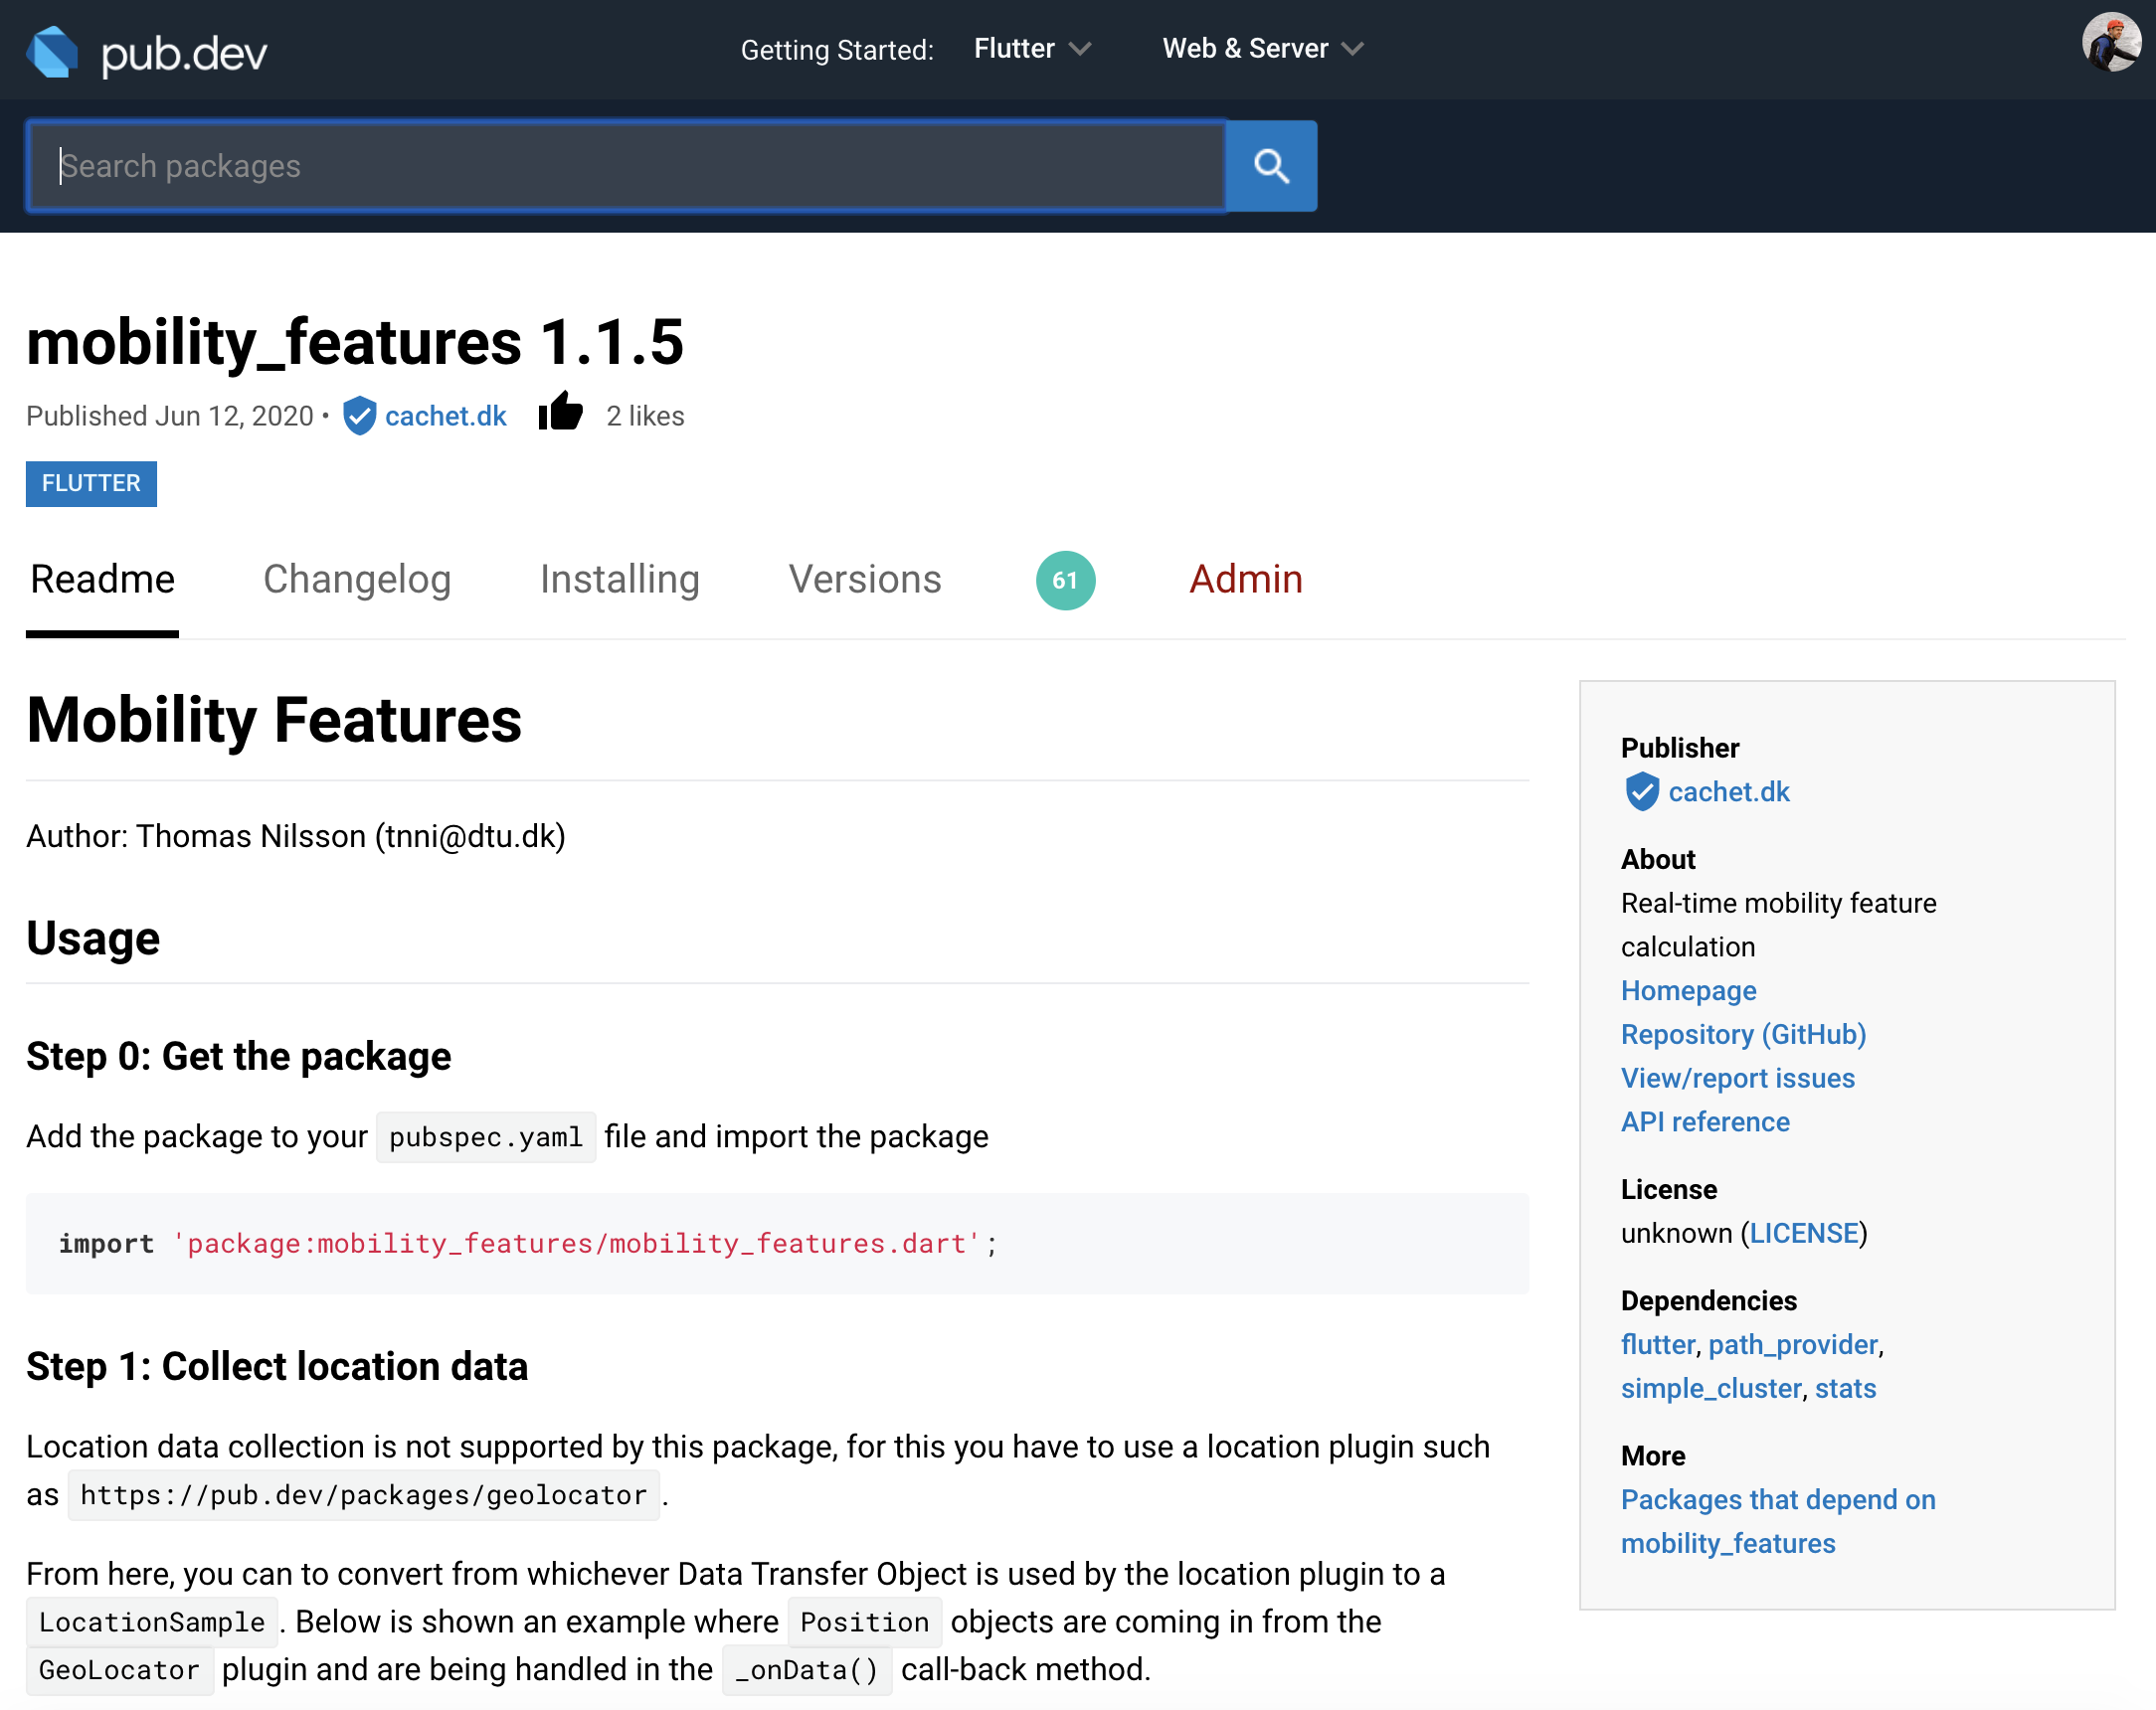
\includegraphics[width=\textwidth]{images/pub.png}
    \caption{The page hosting the Mobility Features Package on www.pub.dev}
    \label{fig:pub-package}
\end{figure}

Publishing automatically generate API documentation by using comments in the code. Normally, comments are made with 2 forward slashes (\textit{//}), but comments made with three forward slashes (\textit{///}) mark the code-block following it with API documentation, i.e. the contents of the comment. 

\begin{figure}
    \centering
    \begin{minted}{dart}
        /// A [LocationSample] holds a 2D [GeoPosition] spatial data point
        /// as well as a [DateTime] value s.t. it may be temporally ordered
        class LocationSample implements _Serializable, _Geospatial {...}
    \end{minted}
    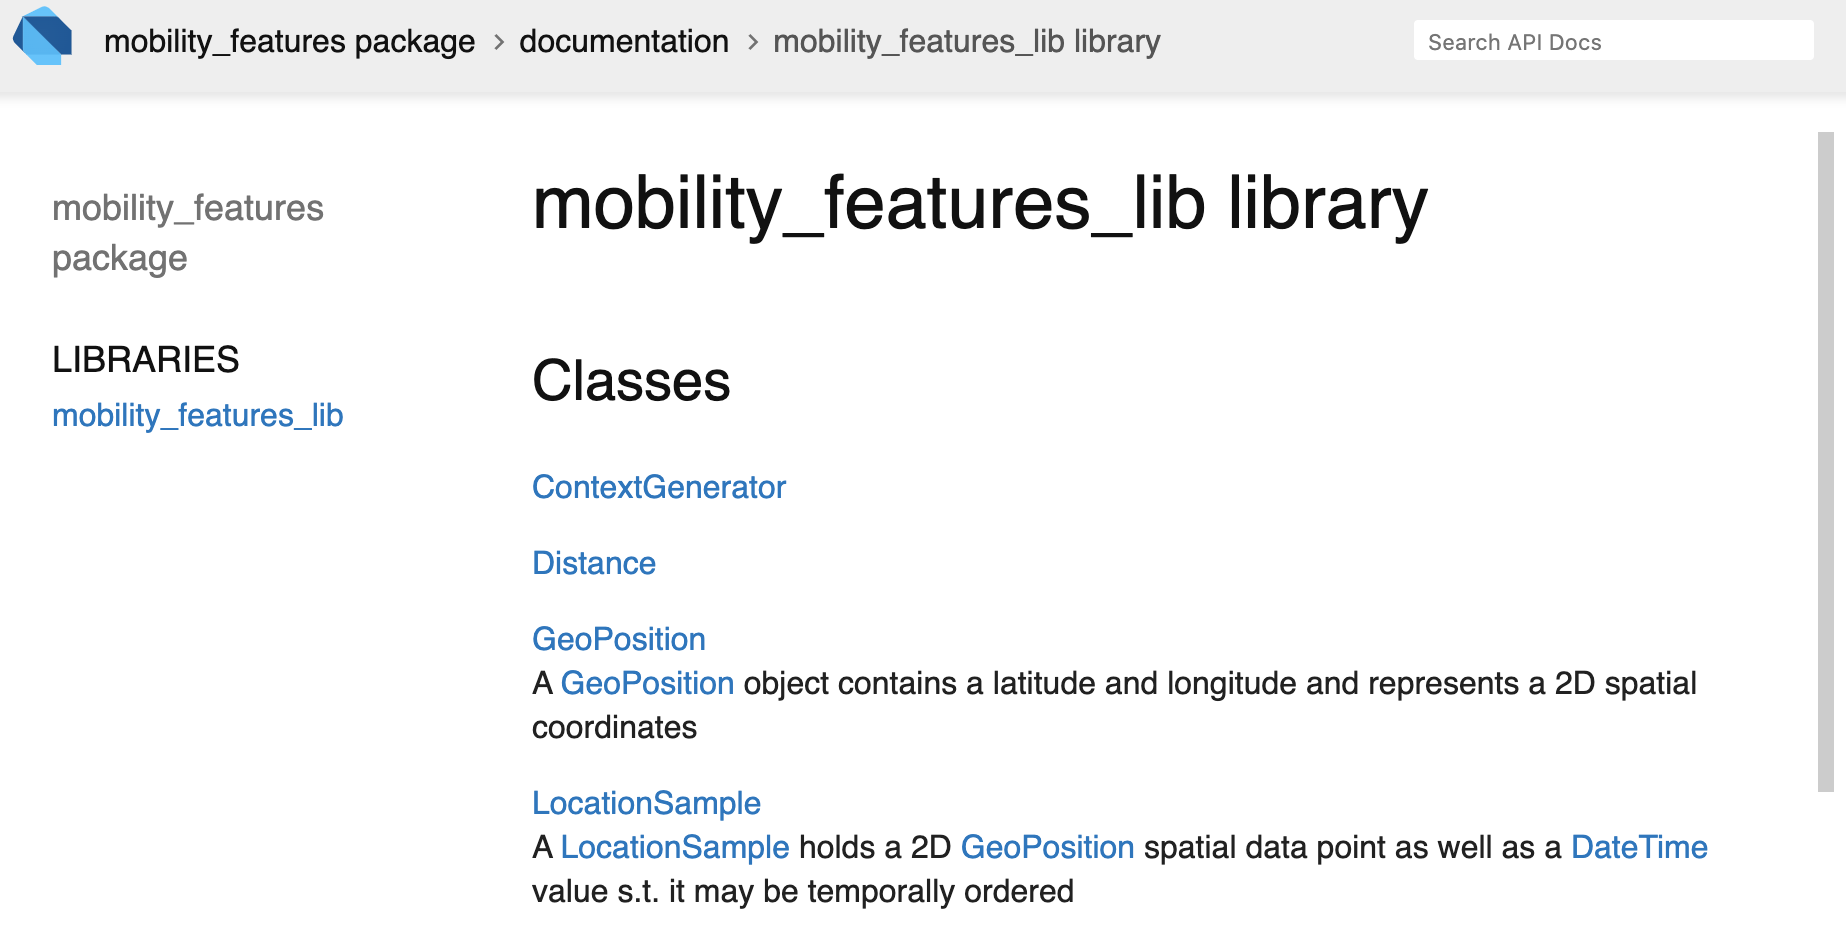
\includegraphics[width=\textwidth]{images/docs.png}
    \caption{The API comments for the source code of a Location Sample (top) and the auto generated documentation hosted on the Pub (bottom)}
    \label{fig:api-docs}
\end{figure}


\section{Package Implementation}
The package was implemented in Flutter according to the design in Chapter \ref{chapter:04} in which a series of components and the overall data model was outlined. This section will go through selected examples of source code as well as the general principles applied, to achieve the specified design, when implementing in Flutter and Dart.

\subsection{Private and Public Access}
In most objective oriented languages, such as Dart, the safest way to use fields in classes is to make them private, and to implement a parameter-less 'getter' method for retrieving the value, and a 'setter' method which takes in the new value as its parameter. In the Dart programming language, a field is declared private by having the the underscore prefix, i.e. \verb|routineIndex| becomes \verb|_routineIndex|, and the corresponding getter method is declared with \verb|get| and is simply called the \verb|routineIndex|:

\begin{minted}{dart}
class MobilityContext {

  double _routineIndex;
  ...
  double get routineIndex {
    return _routineIndex;
  }
}
\end{minted}

This results in an easy-to-read syntax when getting the value of the field, which looks like this:

\begin{minted}{dart}
MobilityContext c = MobilityContext(...);
print(c.routineIndex);
\end{minted}

The same concept can be applied to a constructor as well as the whole class. A public constructor is declared as:
\begin{minted}{dart}
GeoPosition(this._latitude, this._longitude);
\end{minted}

With the private equivalent being:

\begin{minted}{dart}
GeoPosition._(this._latitude, this._longitude);
\end{minted}

A private constructor allows the class to be publicly \textit{available} but not publicly \textit{instantiable}. For classes the underscore prefix is used for the class name, to make it private, similar to field, i.e. \verb|class HourMatrix| becomes \verb|class _HourMatrix|.

On the note of constructors, this package makes use of factory constructors which are effectively just methods which generate an object using the normal constructor. A factory constructor may be used to construct an object from JSON data, where each relevant field is extracted from the JSON data and passed onto the real constructor. A factory constructor is defined as follows:
\begin{minted}{dart}
factory Stop._fromLocationSamples(...) {
	return Stop._(...);
}
\end{minted}

\subsection{Domain Model Implementation}
All the components specified in the Domain Model Chapter \ref{chapter:04} were implemented with their repsective relations to each other. As specified in the component diagram \ref{fig:component-diagram} the only component with a public-facing constructor was LocationSample, and by transitivity, also GeoPosition. This is done, as mentioned, to allow the user instantiate a LocationSample with data from a given Location DTO. The GeoPosition class a field for the latitude and one for the longitude and a fundamental class used by the GeoSpatial interface. The interface is a private abstract class which means it is only visible internally in the package library.

\begin{minted}{dart}
abstract class _Geospatial {
  GeoPosition get geoPosition;
}
\end{minted}

This interface allows other classes to promise the Dart compiler that it has a GeoPosition field which allows it to be compared to other classes which implement the same interface. In Dart interfaces and abstract classes are one and the same thing, and the \textit{abstract class} keyword is used for implementing them. The GeoPosition class even implements this interface since a GeoPosition object itself has a GeoPosition. This may seem superfluous, but will come in handy when finding Stops.

\begin{minted}{dart}
class GeoPosition implements _Serializable, _Geospatial {
  double _latitude;
  double _longitude;

  GeoPosition(this._latitude, this._longitude);

  GeoPosition get geoPosition => this;
  double get latitude => _latitude;
  double get longitude => _longitude;
}
\end{minted}

\subsection{Storing and Loading Data}
The storing and loading of data, which includes Location Samples, Stops and Moves happen through the MobilitySerializer class. This class allows classes which implement the Serializable interface to be serialized and de-serialized. Just like the GeoSpatial interface, the Serializable interface is also implemented as a private abstract class only used internally in the package library. The interface contains a method for serializing a class to JSON, named \verb|toJson()| which takes no parameters and produces a HashMap of Strings to the dynamic, the dynamic type meaning any type. This is the Dart equivalent of a JSON object. Another method the interface forces other classes to implement is the deserialization method \verb|fromJson(json)| which takes a JSON object as parameter and creates a runtime object of the given type, from the JSON object. The implemention of this method is left to the individual classes implementing the interface which is done by extracting data from the JSON object.

\begin{minted}{dart}
abstract class _Serializable {
  Map<String, dynamic> _toJson();

  _Serializable._fromJson(Map<String, dynamic> json);
}
\end{minted}

The MobilitySerializer class is a generic which allows the type \verb|E| to be specified later, with \verb|E| referring to either an Location Sample, Stop or Move which all implement the Serializable interface. The MobilitySerializer is constructed using a reference to a File object. The File object is used for storing the data of the given type i.e. Location Samples are stored one file, Stops in another and Moves in a third.

\begin{minted}{dart}
class MobilitySerializer<E> {
  File file;
  
  MobilitySerializer._(this.file) {
    bool exists = file.existsSync();
    if (!exists) {
      flush();
    }
  }
  
  Future<void> flush() async =>
      await file.writeAsString('', mode: FileMode.write);
\end{minted}

When initialized, it is checked whether or not the specified file exists, and if not the \verb|flush| method is called, which simply writes an empty string to the file, overriding any content, which has the effect of creating the file, should it not already exist. A concrete example of instantiated the MobilitySerializer for Stops is shown below, where \textit{stops.json} refers to the file in which Stops should be stored.

\begin{minted}{dart}
MobilitySerializer<Stop> stopSerializer =
        MobilitySerializer<Stop>._(await _file('stops.json'));
\end{minted}

For storing data the \verb|save| method is used which takes in a list of objects which all implement the Serializable interface. Each element in the list is serialized via its \verb|toJson| method and concatenated into one big string separated by a delimiter token, and this string is then written to the specific file of the MobilitySerializer object.

\begin{minted}{dart}
Future<void> save(List<_Serializable> elements) async {
  String jsonString = "";
  for (_Serializable e in elements) {
    jsonString += json.encode(e._toJson()) + delimiter;
  }
  await file.writeAsString(jsonString, mode: FileMode.writeOnlyAppend);
}
\end{minted}

Loading works in the reverse order, where the contents of the specified file is loaded into a string, the string is then split into elements using the delimiter token and each of these elements is turn de-serialized using the \verb|fromJson| method.  For deciding which type to de-serialize the elements into, a switch statement is used that checks the type of \verb|E| which is specified when the MobilitySerializer object is instantiated.

\begin{minted}{dart}
Future<List<_Serializable>> load() async {
    String content = await file.readAsString();

    List<String> lines = content.split(delimiter);

    Iterable<Map<String, dynamic>> jsonObjs = lines
        .sublist(0, lines.length - 1)
        .map((e) => json.decode(e))
        .map((e) => Map<String, dynamic>.from(e));

    switch (E) {
      case Move:

        return jsonObjs.map((x) => Move._fromJson(x)).toList();
      case Stop:

        return jsonObjs.map((x) => Stop._fromJson(x)).toList();
      default:

        return jsonObjs.map((x) => LocationSample._fromJson(x)).toList();
    }
  }
\end{minted}

Ideally, the switch statement could have been replaced by the following one-liner:
\begin{minted}{dart}
return jsonObjs.map((x) => E.fromJson(x)).toList();
\end{minted}

However, this relies on the language feature called reflection \footnote{\url{https://www.javaworld.com/article/2075801/reflection-vs--code-generation.html}} which allows the compiler to infer the type of \verb|E| at compile-time. However, Dart does not support \textit{reflection} which makes this impossible.

\subsection{Finding Intermediate Features}
Finding the intermediate features Stops, Moves and Places were done according to the algorithms described in Chapter \ref{chapter:03}. 

\subsubsection{Finding Stops}
The Stop class has two constructors: A factory constructor which takes a set of LocationSamples from which the centroid of the set is computed, as well as the earliest timestamp, which will be the arrival time, and the latest timestamp which will be the departure time. After these attributes are found, the normal constructor is used.

\begin{minted}{dart}
  factory Stop._fromLocationSamples(List<LocationSample> locationSamples,
      {int placeId = -1}) {
      
    GeoPosition center = _computeCentroid(locationSamples);
    return Stop._(center, locationSamples.first.datetime, locationSamples.last.datetime,
        placeId: placeId);
  }
\end{minted}

The normal constructor uses a GeoPosition, in addition to an arrival and departure time. A place ID may also be specified at construction, but often it is not yet known at construction time hence it is optional.

\begin{minted}{dart}
  Stop._(this._geoPosition, this._arrival, this._departure, {this.placeId = -1});
\end{minted}

The Stop algorithm takes a List of LocationSamples as input, and uses two while-loops, and two pointers (\textit{start} and \textit{end}) which delimit a subset of the input data we are currently considering with the outer loop. Every time the outer loop moves, the \textit{start} pointer is moved past the end pointer, in order to skip already seen data. The inner loop is responsible for moving the \textit{end} pointer: With each iteration of the inner loop, the centroid of the current subset is computed. If the distance from this centroid to the latest added sample is within the given \verb|stopRadius| parameter, then the subset is expanded by incrementing the \textit{end} pointer., and the process is continued. Otherwise the inner loop terminates and a Stop is created from the subset. The Stop is created without a Place ID, since Places have not yet been identified. In addition, Stops with a duration shorter than the duration specified by the \verb|stopDuration| parameter are removed since they are noisy. This is an addition to the algorithms previously described and is mostly used due to the very high sampling frequency and likely won't be necessary in the general case.

\begin{minted}{dart}
  int start = 0;
  while (start < n) {
    int end = start + 1;
    List<LocationSample> subset = data.sublist(start, end);
    GeoPosition centroid = _computeCentroid(subset);

    while (
        end < n && Distance.fromGeospatial(centroid, data[end]) <= stopRadius) {
      end += 1;
      subset = data.sublist(start, end);
      centroid = _computeCentroid(subset);
    }
    Stop s = Stop._fromLocationSamples(subset);
    stops.add(s);

    start = end;
  }
\end{minted}

The distance calculation \verb|Distance.fromGeospatial(centroid, data[end]) <= stopRadius)| is carried out using the \verb|GeoSpatial| interface previously mentioned. The distance function \verb|fromGeoSpatial| takes two objects which implement the interface and unpacks the latitude and longitude from these objects. The haversine distance can then be computed afterwards.

\begin{minted}{dart}
class Distance {
  static double fromGeospatial(_Geospatial a, _Geospatial b) {
    return fromList(
        [a.geoPosition._latitude, a.geoPosition._longitude],
        [b.geoPosition._latitude, b.geoPosition._longitude]);
  }

  static double fromList(List<double> p1, List<double> p2) {
    /// Haversine implementation
  }
}
\end{minted}

\subsubsection{Finding Moves}
The Move class has two constructors which are both private. Common for both constructors is that they take two Stops as arguments, with argument being either a path of Locaiton Samples or a Distance, i.e. a double. The factory constructor called \verb|_fromPath| calculates the distance of the path and then uses the normal constructor for create a Move. 
\begin{minted}{dart}
  factory Move._fromPath(Stop a, Stop b, List<LocationSample> path) {
    double d = _computePathDistance(path);
    return Move._(a, b, d);
  }
\end{minted}

\begin{minted}{dart}
  Move._(this._stopFrom, this._stopTo, this._distance);
\end{minted}
The normal constructor is used for de-serialization whereas the factory constructor is used to create a Move given two Stops and the path of samples between them.

The algorithm for finding Moves takes a List of Location Samples and the Stops found from the samples as input. The algorithm first checks if the set of Stops is empty, and if so returns an empty set of Moves. If however the set of Stops is not empty, then two 'fake' Stops are created and added to the set of Stops. These two additional stops are created from the first and last element in the set of Location Samples. For each Stop in the set of Stops, it is calculated which samples lie in between the current and next Stop. A Move is then created using the current Stop, the next Stop and the path between. 

\begin{minted}{dart}
  Stop first = Stop._fromLocationSamples([data.first]);
  List<Stop> allStops = [first] + stops;

  if (data.first != data.last) {
    Stop last = Stop._fromLocationSamples([data.last]);
    allStops.add(last);
  }

  for (int i = 0; i < allStops.length - 1; i++) {
    Stop cur = allStops[i];
    Stop next = allStops[i + 1];
    List<LocationSample> samplesInBetween = data
        .where((d) =>
            cur.departure.leq(d.datetime) && d.datetime.leq(next.arrival))
        .toList();

    moves.add(Move._fromPath(cur, next, samplesInBetween));
  }
\end{minted}

The mentioned 'fake' Stops is an addition to the definition in Chapter \ref{chapter:03}. They are created to avoid situations in which tracking was started while moving, in this case no Moves are created before the user is stationary for some time, and Stops are found. This situation will likely not be very common, but was found during self-study and therefore deemed worthy of covering. The extra Stops are only used for finding moves and will not be used for finding Places.

\subsubsection{Finding Places}
The Place class only has one normal constructor which takes an ID (an integer) and a List of Stops. 
\begin{minted}{dart}
Place._(this._id, this._stops);
\end{minted}

The Place algorithm takes a set of Stops for a given period, i.e. Stops over multiple days. The DBSCAN algorithm \cite{density-based-1996} is used to find clusters in the Stops and label each Stop with a cluster ID, this is the place ID previously discussed. Once the labels are computed the Stops are grouped by their Place ID, and a for each group a Place object is created with the group label and the Stops contained in the group. Lastly, the \verb|placeId| attribute for each Stop in the group is set to the group label.

\begin{minted}{dart}
  DBSCAN dbscan = DBSCAN(
      epsilon: placeRadius, minPoints: 1, distanceMeasure: Distance.fromList);
  List<List<double>> stopCoordinates =
      stops.map((s) => ([s.geoPosition.latitude, s.geoPosition.longitude])).toList();

  dbscan.run(stopCoordinates);

  Set<int> clusterLabels = dbscan.label.where((l) => (l != -1)).toSet();

  for (int label in clusterLabels) {
    List<int> indices =
        stops.asMap().keys.where((i) => (dbscan.label[i] == label)).toList();

    List<Stop> stopsForPlace = indices.map((i) => (stops[i])).toList();

    Place p = Place._(label, stopsForPlace);
    places.add(p);

    stopsForPlace.forEach((s) => s.placeId = p._id);
  }
\end{minted}

\subsection{Comuting Features}
A Mobility Context object represents features for a given date. The class has private constructor which takes a List of Stops and Moves from today, and a List of Places from the current period, i.e. the last 28 days including today. When the class is instantiated the date of today is automatically inferred, if not provided through the date parameter, which is an optional parameter. This parameter can be overridden in the case of unit testing for specific dates or if the programmer wishes to compute a Mobility Context for a date in the past.

\begin{minted}{dart}
MobilityContext._(this._stops, this._allPlaces, this._moves,
  {this.contexts, this.date}) {
  _timestamp = DateTime.now();
  date = date ?? _timestamp.midnight;
}
\end{minted}

The other optional parameters is a List of Mobility Contexts is used for computing the Routine Index - how this is achieved will be explained later in this section. The 'derived' features are implemented as doubles (except for Number of Places which is an integer) and are fields in the Mobility Context class. All of these features are accessed via getters, which retrieve the value of the field.

\begin{figure}
    \centering
    \begin{minted}{dart}
    class MobilityContext {
    	// Field
    	double _routineIndex;
     
     	// Getter
        double get routineIndex {
        	return _routineIndex;
        }
    }
    \end{minted}
    \caption{The getter method for a feature field}
    \label{fig:feature-getter}
\end{figure}

\subsubsection{Lazy Evaluation}
A \textit{getter} method for a given feature should reflect that the feature that is to be retrieved requires minimal computation (i.e. 'getting'), and therefore the feature computation should not take place in the getter method. However there is a middle way, since the given feature needs to be computed only once to be evaluated, which allows us to keep the getter syntax. This middle way is \textit{lazy evaluation} \footnote{\url{https://www.martinfowler.com/eaaCatalog/lazyLoad.html}}, which is the idea of having a field be computed only the first time it is needed, and then stored from then on. In practice this is done by letting the field be initialized to \textit{null}, and checking for \textit{null} in the getter method. If the value is \textit{null} then the feature is calculated and the field's value is updated after the computation and the getter can return the field's value. If the field is not \textit{null} then the feature has already been computed, and can be returned immediately.

\begin{figure}
    \centering
    \begin{minted}{dart}
    class MobilityContext {
        // Field
        double _routineIndex;
        
        // Getter
        double get routineIndex {
            if (_routineIndex == null) {
                _routineIndex = _calculateRoutineIndex();
            }
            return _routineIndex;
        }
    }
    \end{minted}
    \caption{Lazy evaluation of a feature}
    \label{fig:lazy-evaluation}
\end{figure}


\subsubsection{Home Stay Computation}
The derived features are computed according to their definitions in \ref{chapter:03}, using the lazy evaluation template outlined in Figure \ref{fig:lazy-evaluation}. The Home Stay feature is not exception. The algorithm for computing Home Stay uses the Stops of today: First, the total time elapsed today is calculated using the departure timestamp of the last known Stop of today. Next, the Stops are used to identify the home place by constructing an Hour Matrix, and then extracting the \verb|homePlaceId| from the Hour Matrix. Then, the total duration spent at the home Place is calculated by summing the duration of the Stops which belong to the home Place. The Home Stay is then calculated as the time at home divided by the total time elapsed.

\begin{figure}
    \centering
\begin{minted}{dart}
double _calculateHomeStay() {
  // Latest known sample time
  DateTime latestTime = _stops.last.departure;

  // Total time elapsed from midnight until the last stop
  int totalTime = latestTime.millisecondsSinceEpoch -
      latestTime.midnight.millisecondsSinceEpoch;

  // Find todays home id, if no home exists today return -1.0
  _HourMatrix hm = this.hourMatrix;
  if (hm.homePlaceId == -1) {
    return -1.0;
  }

  int homeTime = stops
      .where((s) => s.placeId == hm.homePlaceId)
      .map((s) => s.duration.inMilliseconds)
      .fold(0, (a, b) => a + b);

  return homeTime.toDouble() / totalTime.toDouble();
}
\end{minted}
    \caption{The method for computing the Home Stay feature}
    \label{fig:home-stay-code}
\end{figure}

\subsubsection{Routine Index}
The Routine Index is the most difficult to compute by far. The method for computing this feature inside the Mobility Context class is however quite short, but this is due to all the matrix computations being done in the Hour Matrix class, i.e. the averaging and overlapping of matrices. The algorithm first checks if any contexts are provided if not then the Routine Index should be -1.0. Next, the Hour Matrices for each historic date is computed, and from these the average Hour Matrix is computed. Lastly the Routine Index is found by computing the overlap between the two Hour Matrix of today, and the average Hour Matrix, using the \verb|a.computeOverlap(b)| method of the Hour Matrix class.

\begin{figure}
    \centering
    \begin{minted}{dart}
    double _calculateRoutineIndex() {
      // Require at least 2 days to compute the routine index
      if (contexts == null) {
        return -1.0;
      } else if (contexts.isEmpty) {
        return -1.0;
      }
    
      /// Compute the HourMatrix for each context that is older
      List<_HourMatrix> matrices = contexts
          .where((c) => c.date.isBefore(this.date))
          .map((c) => c.hourMatrix)
          .toList();
    
      /// Compute the 'average day' from the matrices
      _HourMatrix avgMatrix = _HourMatrix.average(matrices);
    
      /// Compute the overlap between the 'average day' and today
      return this.hourMatrix.computeOverlap(avgMatrix);
    }
    \end{minted}
    \caption{The method for computing the Routine Index feature}
    \label{fig:routine-index-code}
\end{figure}


\subsection{Using Historical Data}
Historical  Store collected samples
Load collected samples
Filter collected samples
Data from day $n$ is deleted on day $n+1$ when loading

Load historical stops and moves
Filter stops and moves
Recompute for today, replace with new 
Append the filtered historical with new stops and moves
Store by overwriting existing stops and moves

\subsection{Context Generation}
Context Generator
Static class, does not have a state
References the LocationSample serializer, gives access to the user
Works as interface for computing things without being able to alter the state
Does the computation process
Async, since files need to be stored and loaded
Routine Index



\subsection{Improvements}
Currently the implementation (not the design) requires daily computation
If features are not computed on a given day, then all the data collected on that day will be lost next time features are computed due to being filtered out. Currently the user can avoid this by either computing features every day without fault or specifying the date on which the features are yet to be computed.
The fix is to mark data and not throw it out before stops and moves have been evaluated for those samples
When data is loaded, group by date, and compute stops and moves per date. Only then should the samples be thrown out.

Lazy evaluation should probably not be used, instead compute on initialization since initialization is async

ContextGeneration should be done with an isolate, currently the user needs to use an isolate.
Prevent UI thread from freezingMobilitySerializvi
\section{Using the Package}
This section will be a mirror of the official instructions on how to use the package, as of version \textit{1.2.0}. For getting started, the programmer has to download the package by adding it as a dependency in their \verb|pubspec.yaml| file of the Flutter project and running the following command:

\begin{minted}{sh}
flutter packages get
\end{minted}

Once the dependency has been downloaded it can be imported as follows:

\begin{minted}{dart}
import 'package:mobility_features/mobility_features.dart';
\end{minted}

Features are computed using the 3 lines of code displayed in Figure \ref{fig:code-example-intro}:

\begin{figure}[h]
    \centering
    \begin{minted}{dart}
    /// Collect data with a location plugin
    List<LocationSample> locationSamples = ///

    /// Store data via the package
    await ContextGenerator.saveSamples(locationSamples);
    
    /// Compute Features via the package
    MobilityContext context = await ContextGenerator.generate();
    \end{minted}
    \caption{All the three lines of code necessary for the application developer to write}
    \label{fig:code-example-intro}
\end{figure}

The exact method for arriving at this stage is outlined in the following 4 steps.

\subsection*{Step 1: Collect location data}
Location data collection is, as mentioned, not part of the Mobility Features package. The location plugin can be flexibly chosen by the programmer. An example of such a plugin the \textit{GeoLocator} plugin\footnote{\url{https://pub.dev/packages/geolocator}}. From here, each incoming location object has to be converted to a \verb|LocationSample| via the constructor

Below is shown an example where incoming \verb|Position| objects are coming in from the \textit{GeoLocator} plugin and are being handled after saved to a list, in the \verb|_onData()| call-back method.

\begin{minted}{dart}
List<LocationSample> locationSamples = [];
...

void _onData(Position d) async {
    GeoPosition geoPos = GeoPosition(d.latitude, d.longitude);
    LocationSample sample = LocationSample(geoPos, d.timestamp);
    locationSamples.add(sample);
}
\end{minted}

\subsubsection*{Step 2: Save location data}
The location data must be saved on the device such that it can be used in the future. Saving the data to persistent storage prevents it from being lost should the RAM reset. Given that the programmer has collected the samples in a list, the samples can be serialized using the \verb|save()| method of the MobilitySerializer.

\begin{minted}{dart}
await ContextGenerator.saveSamples(locationSamples)
\end{minted}

Ideally, saving the data is done with a certain interval, such as every time 100 samples are collected. 

\subsection*{Step 3: Compute features}
The Features can be computed using the static class \verb|ContextGenerator| which uses the stored location samples, as well as historic features to compute the features for today.

There most basic computation is done as follows:
\begin{minted}{dart}
MobilityContext context = await ContextGenerator.generate();
\end{minted}

Note: it is not possible to instantiate a MobilityContext object directly. 
It must be instantiated through \verb|ContextGenerator.generate()|.

\subsubsection*{Step 3.1: Compute features with prior contexts}
Should the programmer wish to compute the routine index feature as well, then prior contexts are needed. Concretely, the application needs to have tracked data for at least 2 days, to compute this feature. The generation of a Mobility Context using prior contexts is done by overriding the \verb|usePriorContexts| argument and setting it to \verb|true|.

\begin{minted}{dart}
MobilityContext context = 
    await ContextGenerator.generate(usePriorContexts: true);
\end{minted}

\subsubsection*{Step 3.2: Compute features for a specific date}
By default, a MobilityContextobject uses the current date as a reference to filter and group data, however, should one wish to compute the features for a specific date, then it is possible to do so by overriding the \verb|today| argument and providing the desired date.

\begin{minted}{dart}
DateTime myDate = DateTime(01, 01, 2020);
MobilityContext context = 
    await ContextGenerator.generate(today: myDate);
\end{minted}

\subsection*{Step 4: Get features}
All features are implemented as \textit{getters} for the MobilityContext class and can, therefore, be retrieved using the dot-notation. 

\begin{minted}{dart}
MobilityContext context = // Generate context

List<Place> places = context.places;
List<Stop> stops = context.stops;
List<Move> moves = context.moves;

int numberOfPlaces = context.numberOfPlaces;
double homeStay = context.homeStay;
double entropy = context.entropy;
double normalizedEntropy = context.normalizedEntropy;
double distanceTravelled = context.distanceTravelled;
double routineIndex = context.routineIndex;
\end{minted}



